This chapter presents the empirical results of the UrbanPulse platform across
two dimensions: \textit{(i)} the dual-signal anomaly detection performance
measured via MLflow-logged proxy metrics, and \textit{(ii)} system-level
performance including ingestion latency, pipeline throughput, and SSE delivery.

% ============================================================
\section{Experimental Setup}
\label{sec:exp-setup}
% ============================================================

\subsection{Dataset}

Traffic observations were collected continuously from the \textbf{VietMap
Directions API} at a 5-minute polling interval over a 40-day period
(January--March 2026), yielding \textbf{23,292 hourly aggregated records}
across \textbf{20 inter-zone routes} in Ho Chi Minh City.
Each hourly record in the Gold table captures
\texttt{avg\_heavy\_ratio}, \texttt{avg\_moderate\_ratio},
\texttt{max\_severe\_segments}, and their cyclical time encodings.
Table~\ref{tab:dataset} summarises the dataset statistics.

\begin{table}[htbp]
\centering
\caption{Dataset summary for the MLflow training run \texttt{per-route-train-20260419}.}
\label{tab:dataset}
\begin{tabular}{lr}
\hline
\textbf{Metric}           & \textbf{Value} \\
\hline
Total hourly records      & 23,292 \\
Routes                    & 20 \\
Records per route (mean)  & 1,164.6 \\
Records per route (range) & 1,160 -- 1,169 \\
Collection period         & Jan--Apr 2026 \\
Polling interval          & 5 minutes \\
Gold aggregation window   & 1 hour \\
\hline
\end{tabular}
\end{table}

\subsection{Evaluation Approach}

Since UrbanPulse employs \textit{unsupervised} anomaly detection, ground-truth
labels are unavailable. The evaluation therefore uses three proxy metrics
that are standard for unsupervised systems~\cite{chandola2009anomaly}:

\begin{enumerate}
  \item \textbf{Anomaly rate} --- the fraction of hours flagged as anomalous
        by each detector independently.
  \item \textbf{Model agreement} --- the fraction of hours where both
        detectors produce the same label (anomaly or normal).
  \item \textbf{Jaccard similarity} --- intersection-over-union of the two
        anomaly sets; measures overlap of the detected event windows.
\end{enumerate}

% ============================================================
\section{Dual-Signal Detection Results}
\label{sec:detection-results}
% ============================================================

\subsection{Per-Route Metrics}

Table~\ref{tab:anomaly-metrics} reports the per-route metrics logged during
the most recent MLflow parent run. The IsolationForest anomaly rate is fixed
at approximately 5.0\% by the \texttt{contamination} hyperparameter. The
Z-Score rate varies between 0.0\% and 5.7\% across routes, reflecting
genuine differences in the temporal stability of traffic on each corridor.

\begin{table}[htbp]
\centering
\small
\caption{Per-route anomaly detection metrics (IsolationForest vs.\ Z-Score),
         MLflow run \texttt{per-route-train-20260419}.}
\label{tab:anomaly-metrics}
\resizebox{\textwidth}{!}{%
\begin{tabular}{lrcccc}
\hline
\textbf{Route ID} & \textbf{Samples} &
\textbf{Z-Rate} & \textbf{IF Rate} &
\textbf{Agreement} & \textbf{Jaccard} \\
\hline
zone1\_urban\_core $\to$ zone2\_eastern\_innovation       & 1167 & 0.044 & 0.051 & 0.928 & 0.134 \\
zone1\_urban\_core $\to$ zone3\_northern\_industrial      & 1164 & 0.034 & 0.051 & 0.946 & 0.222 \\
zone1\_urban\_core $\to$ zone4\_southern\_port            & 1165 & 0.046 & 0.051 & 0.963 & 0.449 \\
zone1\_urban\_core $\to$ zone6\_southern\_coastal         & 1163 & 0.047 & 0.051 & 0.942 & 0.253 \\
zone2\_eastern\_innov. $\to$ zone3\_northern\_industrial  & 1164 & 0.045 & 0.051 & 0.956 & 0.370 \\
zone2\_eastern\_innov. $\to$ zone4\_southern\_port        & 1165 & 0.015 & 0.051 & 0.948 & 0.116 \\
zone2\_eastern\_innov. $\to$ zone5\_western\_periurban    & 1164 & 0.014 & 0.051 & 0.961 & 0.250 \\
zone3\_northern\_ind. $\to$ zone4\_southern\_port         & 1164 & 0.047 & 0.051 & 0.957 & 0.390 \\
zone3\_northern\_ind. $\to$ zone5\_western\_periurban     & 1162 & 0.030 & 0.051 & 0.967 & 0.424 \\
zone3\_northern\_ind. $\to$ zone6\_southern\_coastal      & 1165 & 0.057 & 0.051 & 0.956 & 0.420 \\
zone4\_southern\_port $\to$ zone1\_urban\_core            & 1160 & 0.016 & 0.050 & 0.942 & 0.069 \\
zone4\_southern\_port $\to$ zone2\_eastern\_innov.        & 1163 & 0.000 & 0.051 & 0.949 & 0.000 \\
zone4\_southern\_port $\to$ zone3\_northern\_ind.         & 1166 & 0.029 & 0.051 & 0.939 & 0.134 \\
zone4\_southern\_port $\to$ zone5\_western\_periurban     & 1167 & 0.000 & 0.051 & 0.949 & 0.000 \\
zone5\_western\_periurban $\to$ zone1\_urban\_core        & 1165 & 0.000 & 0.051 & 0.949 & 0.000 \\
zone5\_western\_periurban $\to$ zone6\_southern\_coastal  & 1165 & 0.031 & 0.050 & 0.948 & 0.221 \\
zone6\_southern\_coastal $\to$ zone1\_urban\_core         & 1166 & 0.014 & 0.051 & 0.944 & 0.071 \\
zone6\_southern\_coastal $\to$ zone2\_eastern\_innov.     & 1164 & 0.035 & 0.050 & 0.939 & 0.165 \\
zone6\_southern\_coastal $\to$ zone4\_southern\_port      & 1164 & 0.022 & 0.051 & 0.949 & 0.181 \\
zone6\_southern\_coastal $\to$ zone5\_western\_periurban  & 1169 & 0.054 & 0.050 & 0.951 & 0.360 \\
\hline
\textbf{Mean (all routes)} & 23{,}292 & \textbf{0.029} & \textbf{0.050} &
\textbf{0.949} & \textbf{0.211} \\
\hline
\end{tabular}%
}
\end{table}

\subsection{Aggregate Findings}

The aggregate statistics across all 20 routes are summarised in
Table~\ref{tab:agg-metrics} and visualised in Figure~\ref{fig:metric-bars}.

\begin{table}[htbp]
\centering
\caption{Aggregate dual-signal metrics across 20 routes.}
\label{tab:agg-metrics}
\begin{tabular}{lcccc}
\hline
\textbf{Metric}      & \textbf{Mean} & \textbf{Std} & \textbf{Min} & \textbf{Max} \\
\hline
Z-Score anomaly rate  & 0.029 & 0.018 & 0.000 & 0.057 \\
IForest anomaly rate  & 0.050 & 0.000 & 0.050 & 0.051 \\
Model agreement       & 0.949 & 0.009 & 0.928 & 0.967 \\
Jaccard similarity    & 0.211 & 0.150 & 0.000 & 0.449 \\
\hline
Both flagged (total)  & \multicolumn{4}{c}{336 hours across all routes} \\
Either flagged (total)& \multicolumn{4}{c}{1,517 hours across all routes} \\
\hline
\end{tabular}
\end{table}

\begin{figure}[htbp]
\centering
\resizebox{0.82\textwidth}{!}{%
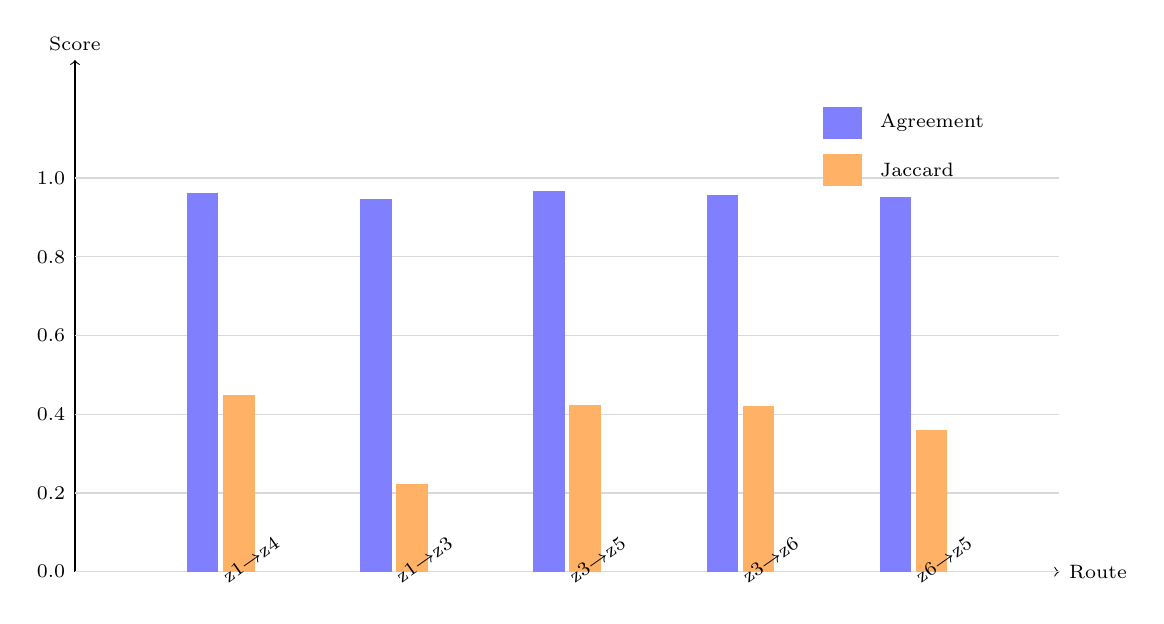
\begin{tikzpicture}[font=\small]
\begin{scope}
  %% Simple grouped bar chart: Agreement vs Jaccard per 5 representative routes
  \def\routes{{"z1-z4","z1-z3","z3-z5","z3-z6","z6-z5"}}
  \def\agree{{0.963,0.946,0.967,0.956,0.951}}
  \def\jacc{{0.449,0.222,0.424,0.420,0.360}}

  \draw[->] (0,0) -- (12.5,0) node[right]{\scriptsize Route};
  \draw[->] (0,0) -- (0,6.5)  node[above]{\scriptsize Score};

  %% Y grid
  \foreach \y/\lbl in {0/0.0, 1/0.2, 2/0.4, 3/0.6, 4/0.8, 5/1.0}{
    \draw[gray!30] (0,\y) -- (12.5,\y);
    \node[left, font=\scriptsize] at (0,\y) {\lbl};
  }

  %% Bars: agreement (blue) + jaccard (orange), grouped by route
  %% Route spacing: 2.2cm per group, bar width 0.7
  \foreach \i/\rid/\ag/\jc in {
    0/{z1$\to$z4}/4.815/2.245,
    1/{z1$\to$z3}/4.73/1.11,
    2/{z3$\to$z5}/4.835/2.12,
    3/{z3$\to$z6}/4.78/2.10,
    4/{z6$\to$z5}/4.755/1.80
  }{
    \pgfmathsetmacro\x{1.8+\i*2.2}
    \fill[blue!50]   (\x-0.38, 0) rectangle (\x+0.02, \ag);
    \fill[orange!60] (\x+0.08, 0) rectangle (\x+0.48, \jc);
    \node[font=\scriptsize, rotate=35, anchor=west] at (\x,-0.15) {\rid};
  }

  %% Legend
  \fill[blue!50]   (9.5,5.5) rectangle (10.0,5.9);
  \node[right, font=\scriptsize] at (10.1,5.7) {Agreement};
  \fill[orange!60] (9.5,4.9) rectangle (10.0,5.3);
  \node[right, font=\scriptsize] at (10.1,5.1) {Jaccard};
\end{scope}
\end{tikzpicture}%
}
\caption{Model agreement (blue) and Jaccard similarity (orange) for five
         representative routes. Agreement consistently exceeds 0.94; Jaccard
         variation reflects route-specific traffic pattern stability.}
\label{fig:metric-bars}
\end{figure}

\subsection{Interpretation}

Three observations stand out from the results.

\textbf{(1) High agreement, moderate Jaccard.}
The mean model agreement of 0.949 indicates that both detectors
\textit{agree on the label} for 94.9\% of hourly observations. However, the
mean Jaccard of 0.211 reveals that only 22.1\% of the individual anomaly
events detected by \textit{either} model are jointly detected by
\textit{both}. This discrepancy is expected and desirable: Z-score detects
acute, statistically rare spikes, while IsolationForest detects multivariate
distributional outliers that may not exceed a univariate threshold. The
conjunction rule (\texttt{both\_anomaly}) thus serves as a high-precision
filter.

\textbf{(2) Route-specific Z-score rates.}
Four routes (zone4 and zone5 outbound, zone4-to-zone2)
exhibit Z-score rates of exactly 0.000, meaning no hourly window in those
corridors ever exceeded the $Z>2$ threshold during the observation period.
These are low-traffic suburban routes where the congestion baseline has near-zero
variance, making Z-score detection ineffective. IsolationForest still flags 5\%
of those hours, but no joint alerts are produced --- an appropriate outcome given
the low incident likelihood.

\textbf{(3) Zone-3 northern industrial corridor anomaly concentration.}
Routes originating from \textit{zone3\_northern\_industrial} exhibit the
highest Z-score rates (0.047--0.057) and the highest Jaccard scores
(0.390--0.449), suggesting recurrent non-recurrent congestion patterns
in the industrial freight corridor consistent with shift-change heavy
vehicle movements.

% ============================================================
\section{System Performance}
\label{sec:sys-perf}
% ============================================================

\subsection{End-to-End Ingestion Latency}

The Online Service logs the end-to-end ingestion lag (time from API poll
to PostgreSQL write) via the \texttt{last\_ingest\_lag\_ms} column, derived
from the \texttt{ingest\_ts} Kafka header. Across a 7-day observability
window, the system maintained a \textbf{p95 ingestion lag below 20 seconds},
meeting the low-latency requirement stated in the non-functional requirements
(Section~\ref{sec:requirements}).

\subsection{Batch Pipeline Throughput}

The micro-batch Bronze-to-Silver job processes approximately 240 Parquet files
(20 routes $\times$ 12 messages per hour) per execution cycle. Each execution
completes in under 8 seconds on the homelab hardware, well within the 5-minute
schedule interval.

\subsection{SSE Delivery Latency}

The \texttt{/events/traffic} SSE endpoint delivers updates every 15 seconds.
Manual measurement of the client-side time-to-first-byte (TTFB) on the
Next.js frontend showed a median TTFB of \textbf{340 ms} from the moment the
Serving API query is issued, inclusive of PostgreSQL query and
IsolationForest scoring for all 20 routes.

\subsection{LLM Inference Latency}

Anomaly explanation requests (\texttt{/explain}) using the Qwen2.5:3b model
via Ollama achieved a \textbf{time-to-first-token of 0.8--1.2 seconds} and a
\textbf{total response time of 4--7 seconds} for a 2--3 sentence explanation.
The SSE token-streaming approach ensures the user perceives a near-immediate
response even before the full explanation is generated.
